\documentclass[10pt]{beamer}

\usepackage{setup}
\usepackage[vlined]{algorithm2e}
\SetAlFnt{\scriptsize}

\title{Time Warp Simulation on Multi-core Processors and Clusters}
\author{
    Douglas A. Weber \\
    Masters Thesis Defense \\
    Advisor: Professor Philip A. Wilsey
}
\institute{University of Cincinnati}
\date{March 8, 2016}

\begin{document}

\begin{frame}
  \titlepage
\end{frame}

\begin{frame}{Discrete Event Simulation}
    \begin{itemize}
        \item Three main components
            \begin{itemize}
                \item State variables
                \item Simulation clock
                \item Pending event set
            \end{itemize}
        \bigskip
        \item Unprocessed events stored in pending event set
        \item Events processed in time stamp order
        \item Simulation clock and state variables updated only when event occurs
    \end{itemize}
\end{frame}

\begin{frame}{Parallel Discrete Event Simulation}

    \begin{columns}[c]

    \begin{column}{0.4\textwidth}
        \begin{itemize}
            \item Model system as a set of Logical Processes (LPs)
            \item Events exchanged between LPs
        \end{itemize}
    \end{column}

    \begin{column}{0.6\textwidth}
        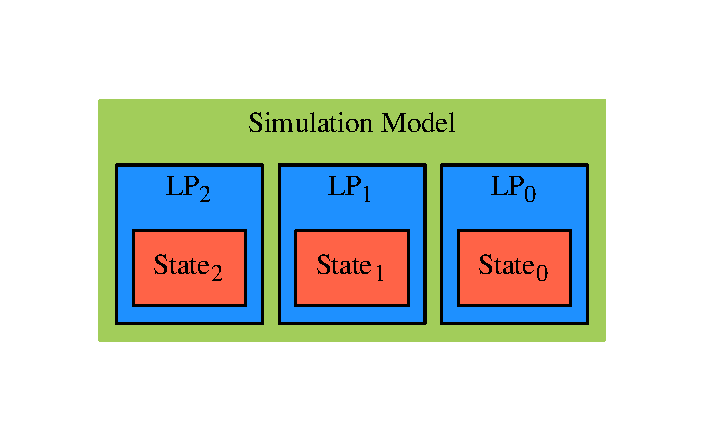
\includegraphics[width=\textwidth]{../figs/graphviz/pdes.pdf}
    \end{column}

    \end{columns}

    \vspace{-\bigskipamount}
    \vspace{-\bigskipamount}
    \begin{block}{Possible Causality Violations}
    \vspace{-\bigskipamount}

        \begin{columns}

        \begin{column}{0.5\textwidth}
            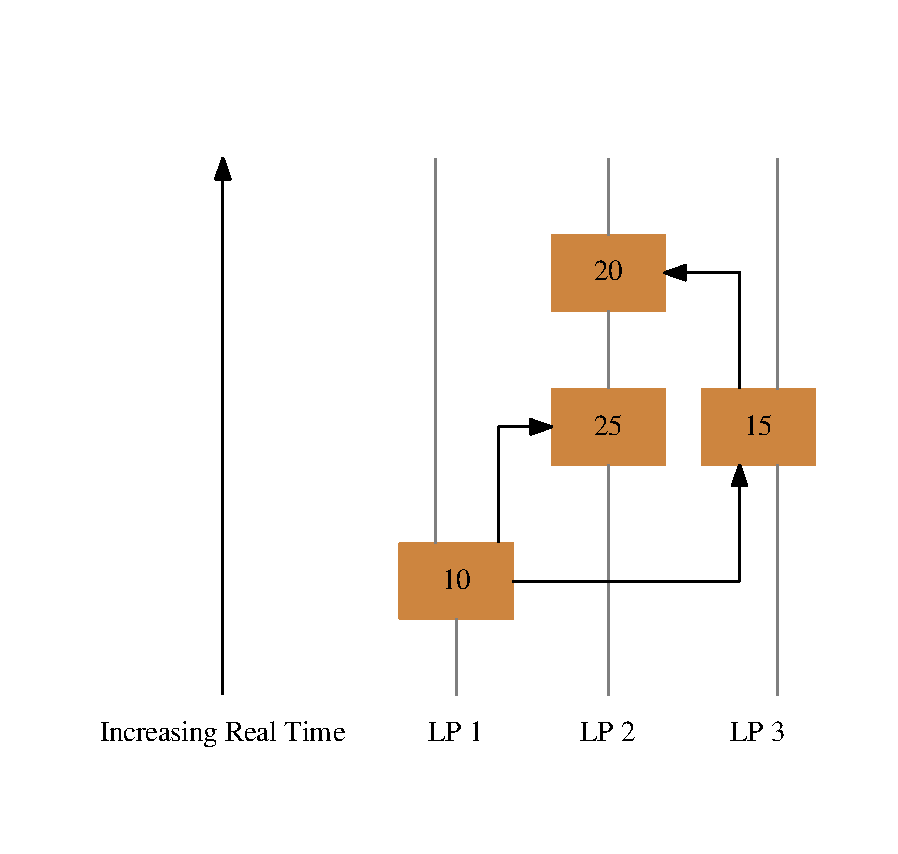
\includegraphics[width=\textwidth]{../figs/graphviz/causality.pdf}
        \end{column}

        \begin{column}{0.5\textwidth}
            \begin{itemize}
                \item Events can be received \emph{and} processed out of order
                  \bigskip
                \item Two solutions
                    \begin{itemize}
                    \item Conservative
                    \item Optimistic
                    \end{itemize}
            \end{itemize}
        \end{column}

        \end{columns}

    \end{block}

\end{frame}

\begin{frame}{Time Warp}
    \begin{block}{Optimistic Mechanism}
        \bigskip
        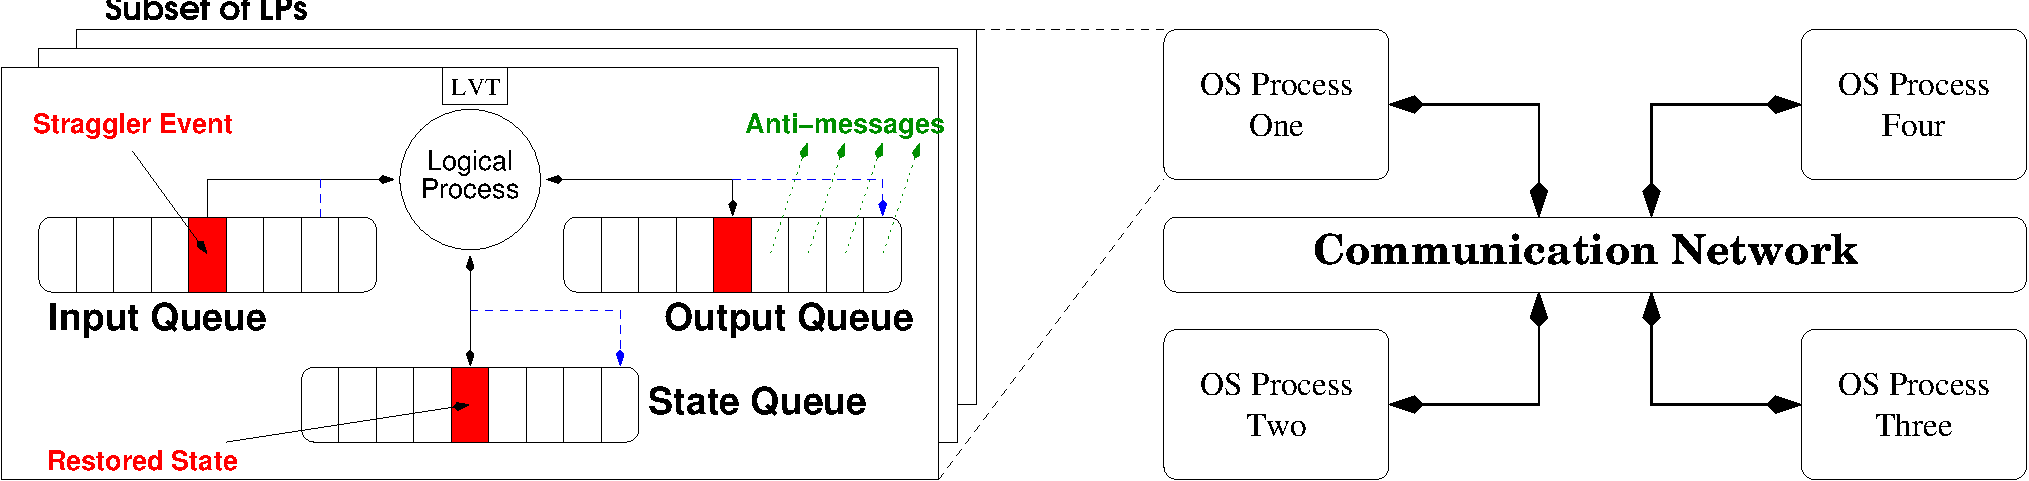
\includegraphics[width=\textwidth]{../figs/timeWarp.pdf}
        \bigskip
        \begin{itemize}
            \item Rollback Mechanism
                \begin{itemize}
                    \item State Restoration, Anti-Messages
                \end{itemize}
            \item Local Virtual Time (LVT) \& Global Virtual Time (GVT)
            \item Fossil Collection
        \end{itemize}
    \end{block}
\end{frame}

\begin{frame}{\textsc{warped2} Process}
        \centerline{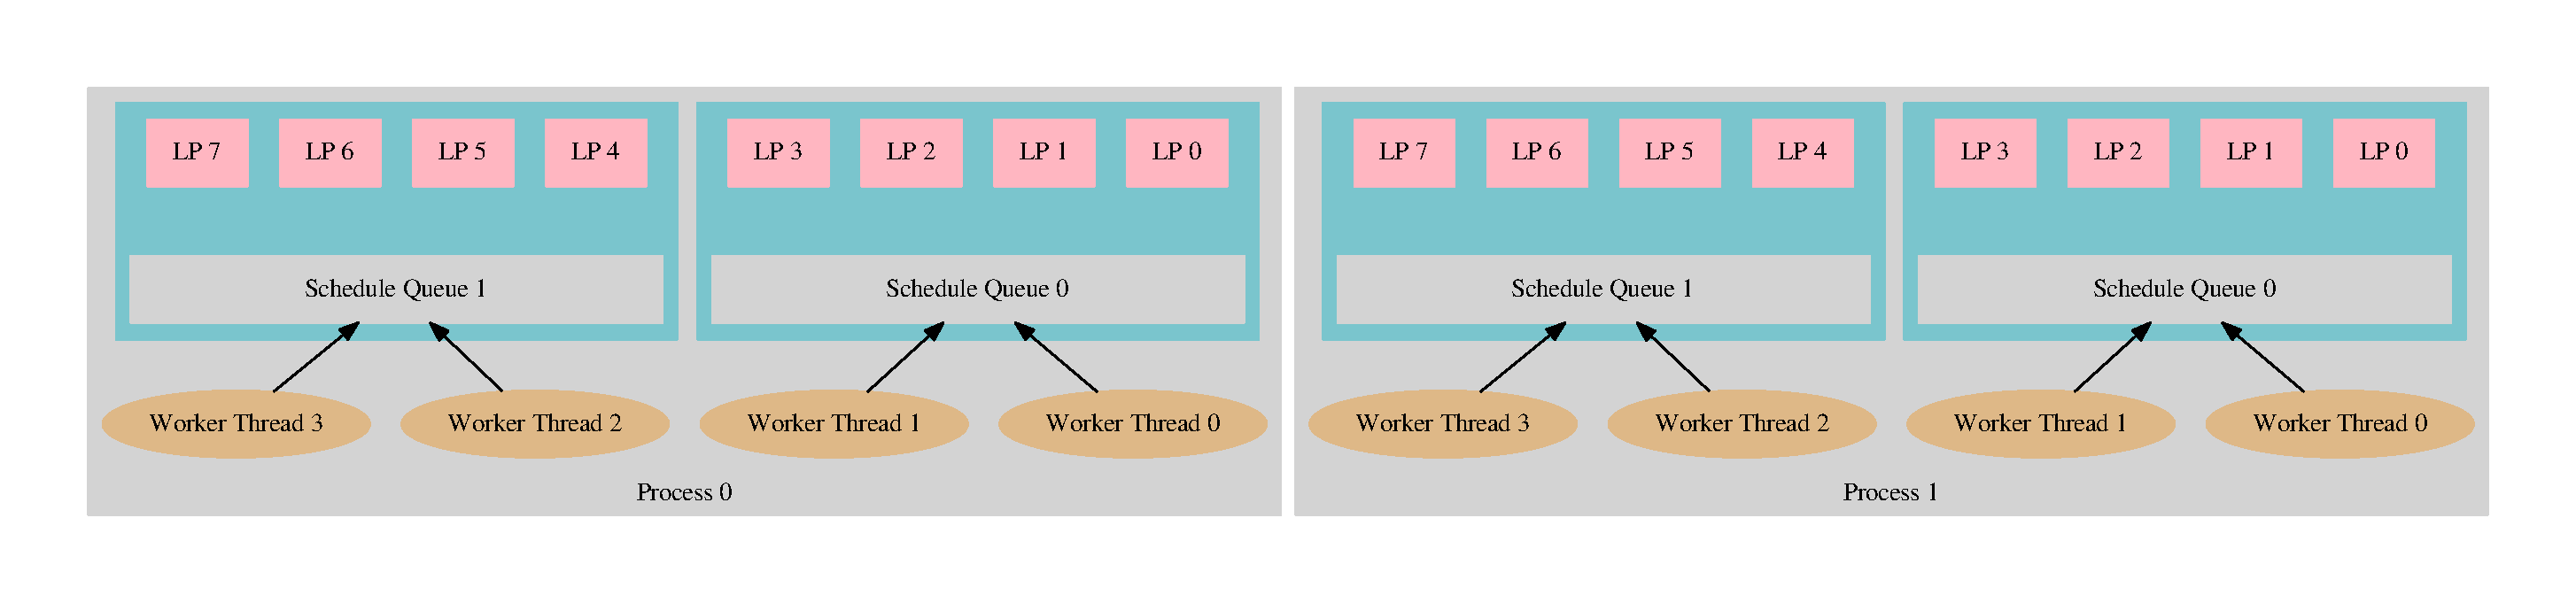
\includegraphics[width=1.2\textwidth]{../figs/graphviz/partitioning.pdf}}
        \begin{itemize}
            \item Worker Threads and Manager Thread
            \item LTSF Queues/Worker Thread: Contention vs Rollbacks
            \item LP Partitioning
        \end{itemize}
\end{frame}

\begin{frame}{Event Scheduling and Processing}
    \begin{columns}

        \begin{column}{0.4\textwidth}

            \begin{block}{Worker Threads}
            \bigskip
            
            \begin{algorithm}[H]
                \DontPrintSemicolon
                \SetKw{Continue}{continue}
                \SetKwFunction{getNextEvent}{getNextEvent}

                \While{termination not detected}{
                    $e \gets \getNextEvent{}$\;
                    $lp \gets$ receiver of $e$\;\;

                    \If{$e <$ last processed event for $lp$}{
                        rollback $lp$\;
                    }
                    \;
                    \If{$e$ is an anti-message}{
                        cancel event with $e$\;
                        schedule new event for $lp$\;
                        \Continue\;
                    }
                    \;
                    process event $e$\;
                    save state of $lp$\;
                    send new events\;
                    \;
                    move $e$ to processed queue\;
                    replace scheduled event for $lp$\;
                }
            \end{algorithm}

            \end{block}

        \end{column}

        \begin{column}{0.6\textwidth}
            \centerline{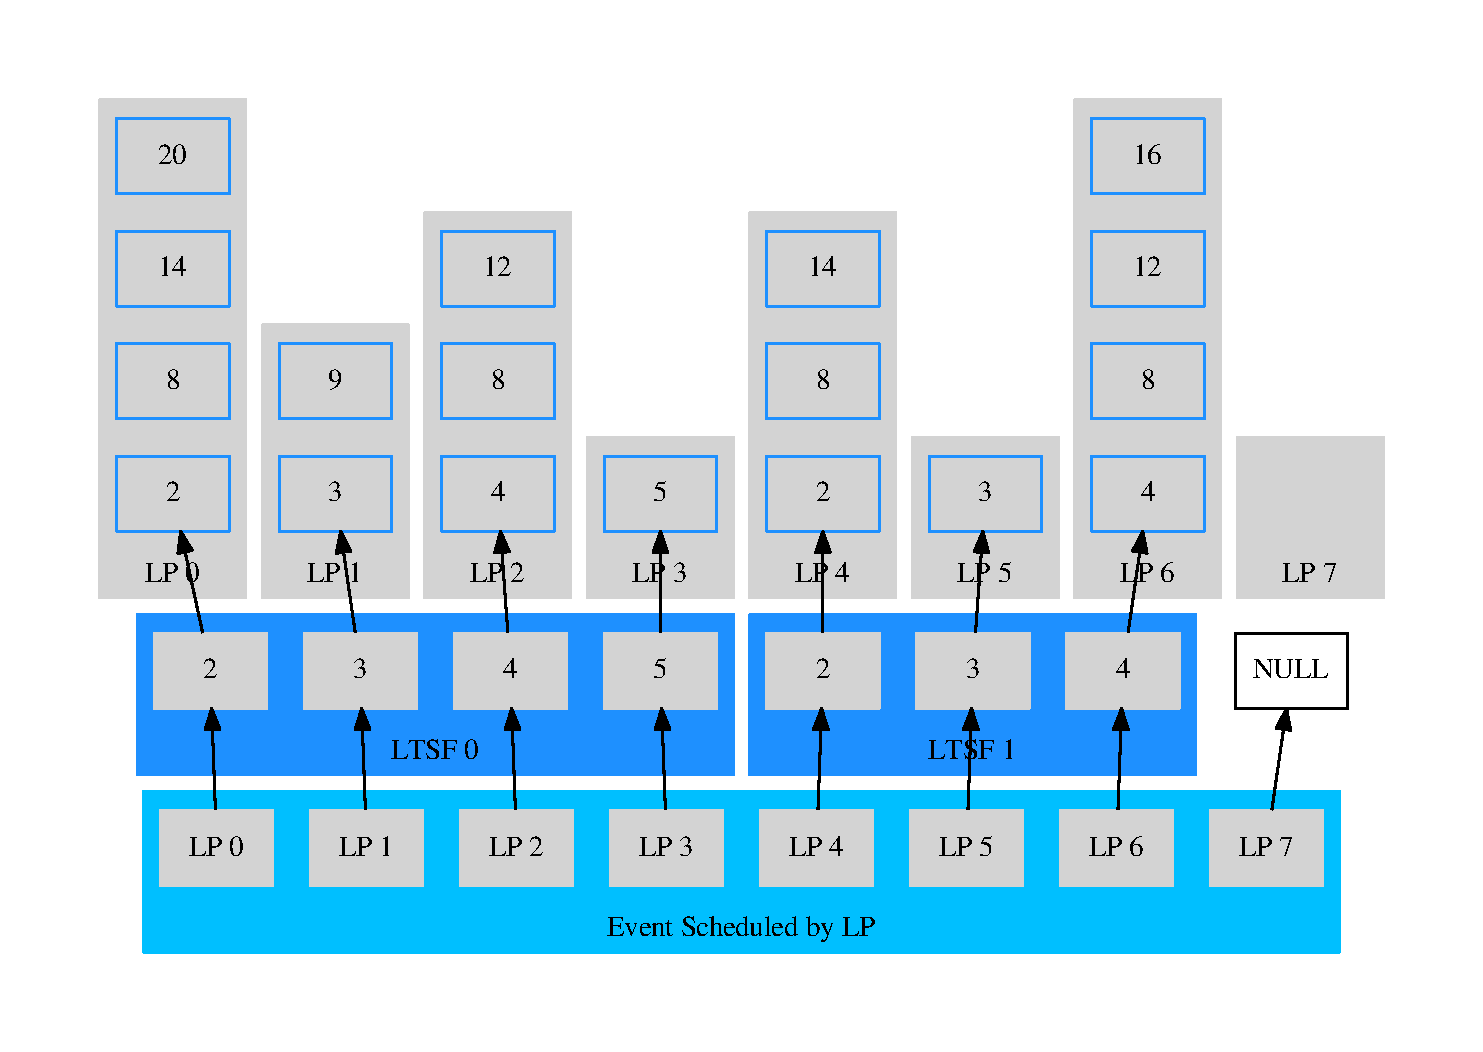
\includegraphics[width=1.35\textwidth]{../figs/graphviz/pending_event_set.pdf}}
            \vspace{-\bigskipamount}
            \vspace{-\bigskipamount}
            \begin{itemize}
                \item Unprocessed and Processed Queues
                \item Scheduling to LTSF
                \item Rollbacks
            \end{itemize}
        \end{column}

    \end{columns}
\end{frame}

\begin{frame}{Sharing LTSF Queues}
  \bigskip
  \bigskip
    \begin{block}{Intel\textsuperscript{\textregistered} Xeon\textsuperscript{\textregistered} X5675 (6 cores/10 worker threads)}\end{block}
    \vspace*{-\medskipamount}
    \begin{minipage}{0.55\textwidth}
        \centerline{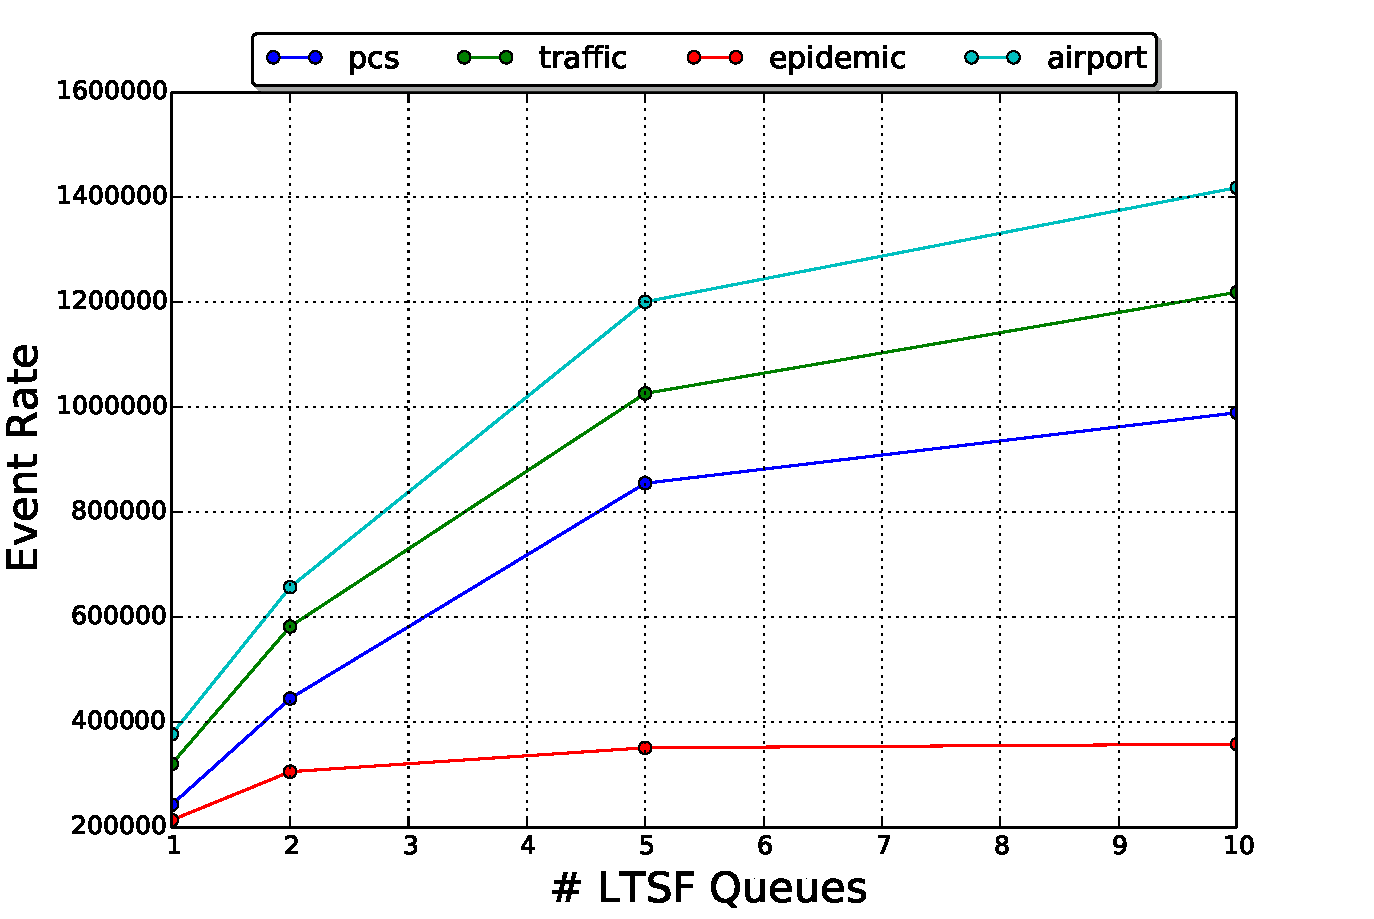
\includegraphics[width=\textwidth]{../figs/pending_event_set/ltsf_event_rate.pdf}}
        \vspace*{-\medskipamount}
        \small{$$EventRate={CommitedEvents \over Runtime}$$}
    \end{minipage}%
    \begin{minipage}{0.55\textwidth}
        \centerline{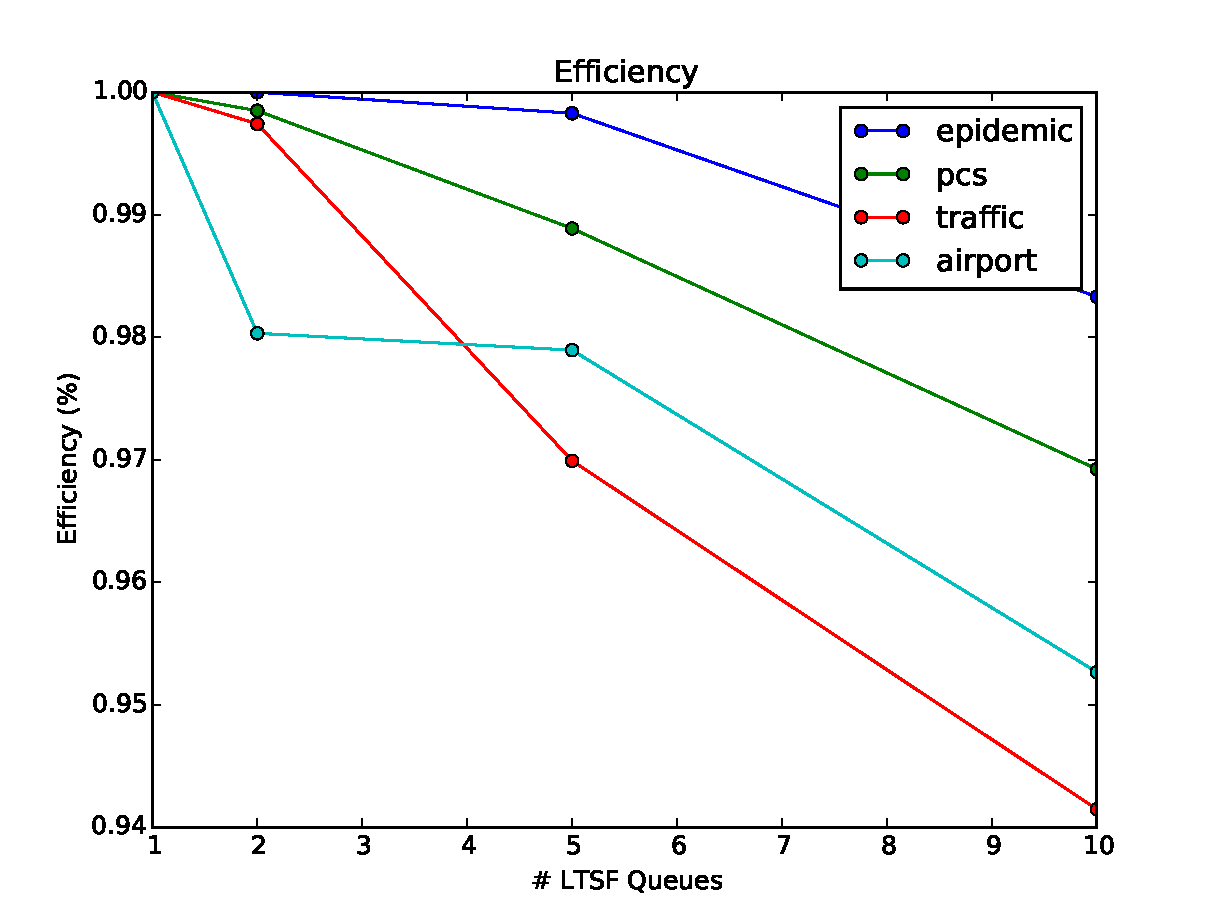
\includegraphics[width=\textwidth]{../figs/pending_event_set/ltsf_efficiency.pdf}}
        \vspace*{-\bigskipamount}
        \small{$$Efficiency={CommittedEvents \over ProcessedEvents}*100 \%$$}
    \end{minipage}
    \medskip
    \begin{block}{Reducing contention more important than reducing rollbacks}\end{block}
\end{frame}

\begin{frame}{Periodic State Saving: Overview}
    \begin{block}{Save state only once every $N$ events}
        \bigskip
        \centering
        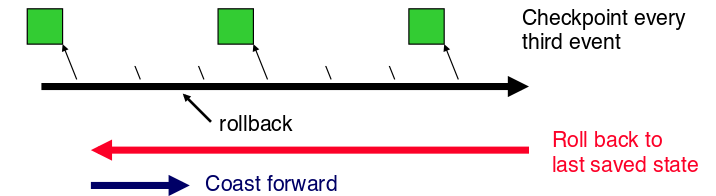
\includegraphics[width=0.6\textwidth]{../figs/pss.png}
        \bigskip
        \begin{itemize}
            \item Not all states available to roll back to
            \item Must ``Coast Forward'' to reproduce state
            \item Increases time to rollback
            \item Decrease time to save states and reduce memory footprint
        \end{itemize}
    \end{block}
\end{frame}

\begin{frame}{Periodic State Saving: SMP Machine}
    \begin{block}{Intel\textsuperscript{\textregistered} Xeon\textsuperscript{\textregistered} X5675 (6 cores/10 worker threads)}
        \bigskip
        \begin{minipage}{0.55\textwidth}
            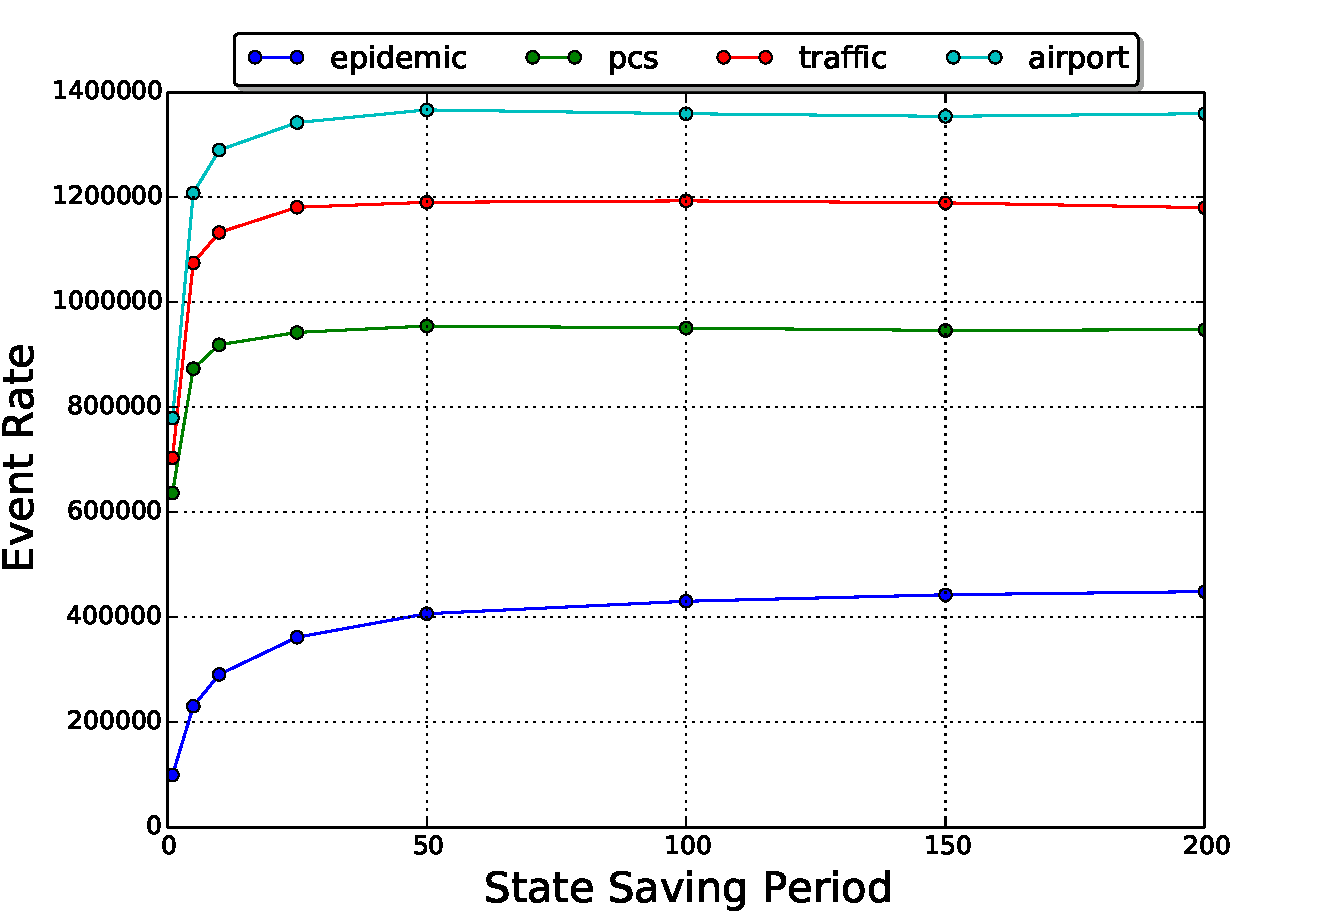
\includegraphics[width=\textwidth]{../figs/state_saving/bc/eventrate.pdf}
        \end{minipage}%
        \begin{minipage}{0.55\textwidth}
            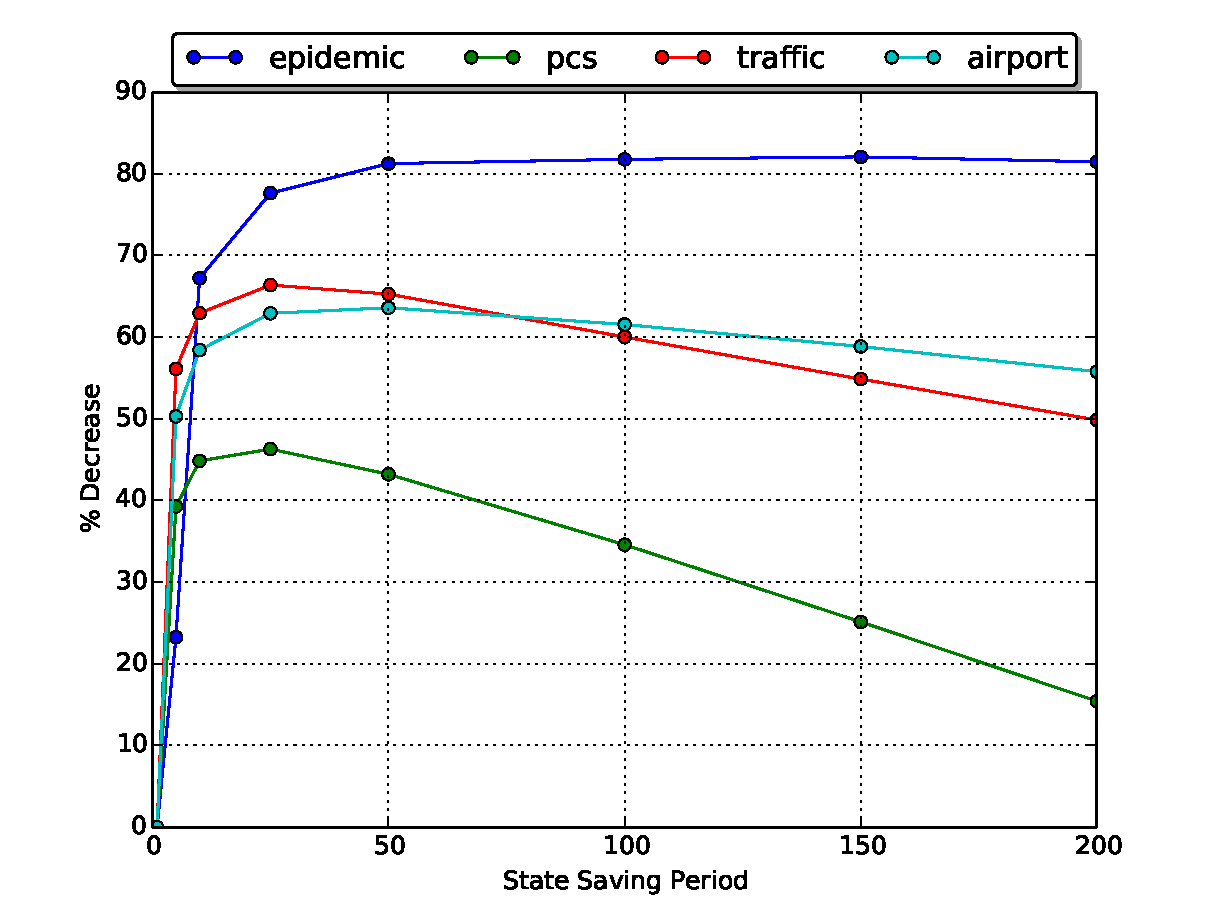
\includegraphics[width=\textwidth]{../figs/state_saving/bc/percent_memory_decrease.pdf}
        \end{minipage}
    \end{block}
\end{frame}

\begin{frame}{Periodic State Saving: Cluster}
    \begin{block}{Intel\textsuperscript{\textregistered} Xeon\textsuperscript{\textregistered} E5410 (8 nodes)}
        \smallskip
        \begin{minipage}{0.55\textwidth}
            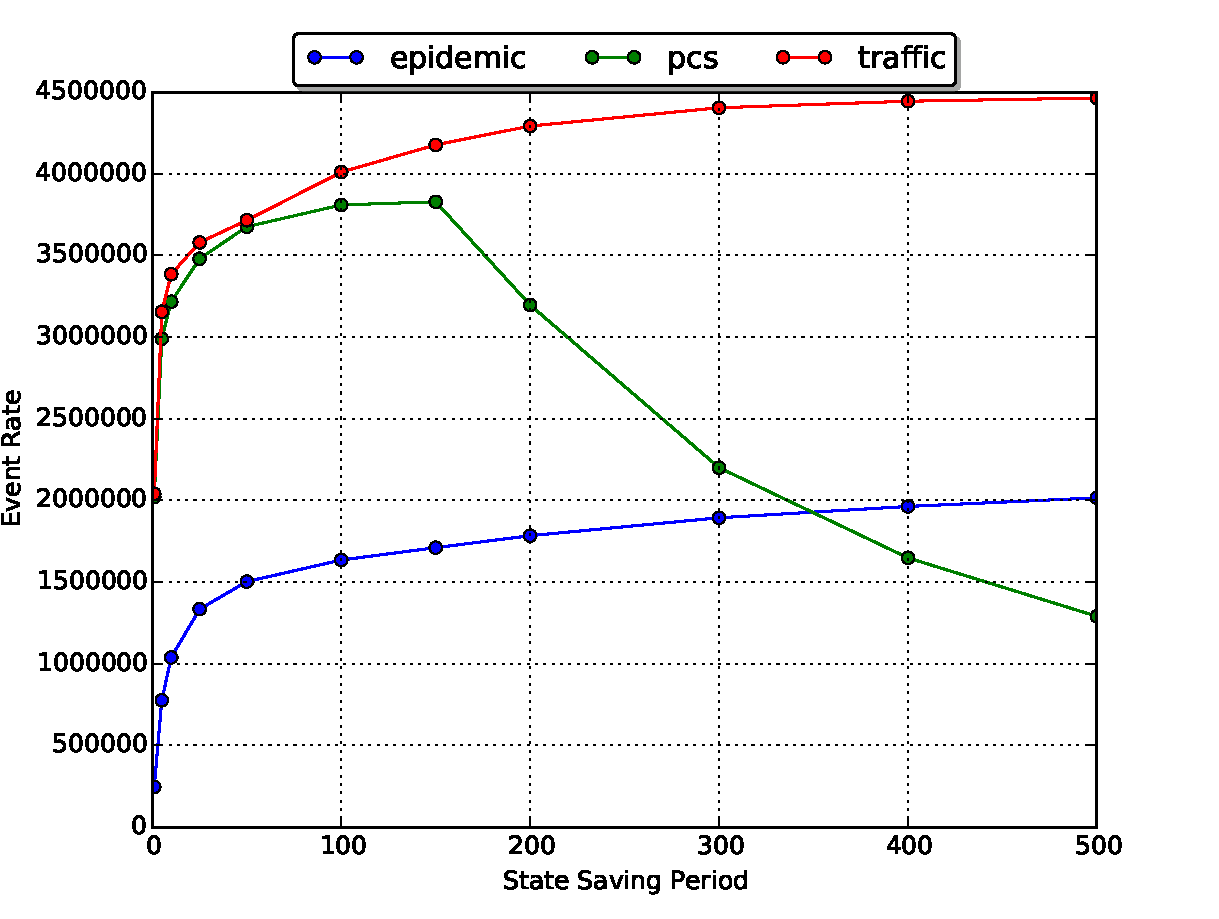
\includegraphics[width=\textwidth]{../figs/state_saving/beowulf/eventrate_500.pdf}
        \end{minipage}%
        \begin{minipage}{0.55\textwidth}
            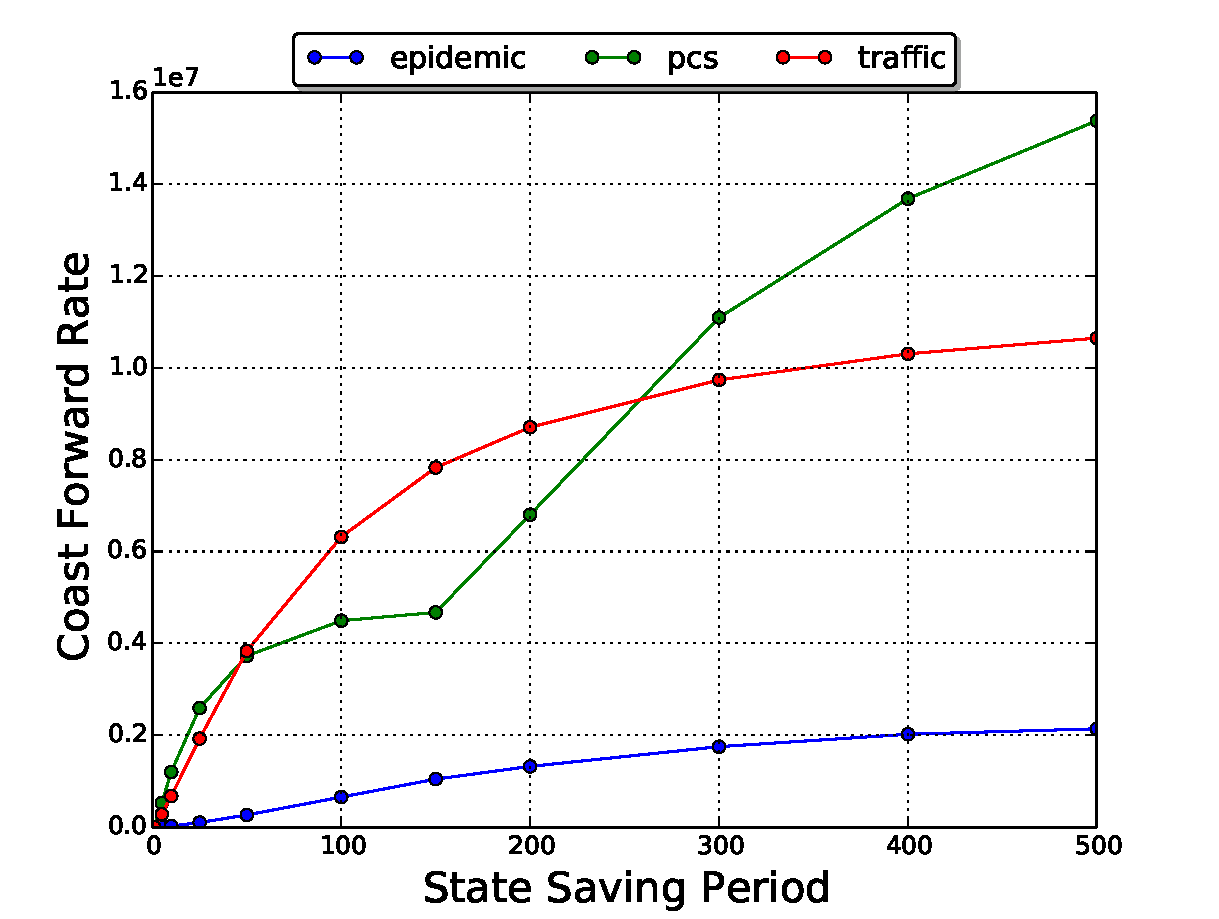
\includegraphics[width=\textwidth]{../figs/state_saving/beowulf/cf_rate_500.pdf}
        \end{minipage}
    $$ CoastForwardRate = {CoastForwardEvents \over Rollbacks} * RollbackRate $$
    \end{block}
\end{frame}

\begin{frame}{Communication Model}
    Shared Memory vs Message Passing
    \begin{itemize}
        \item Sending Events, GVT, Termination
    \end{itemize}
    \centerline{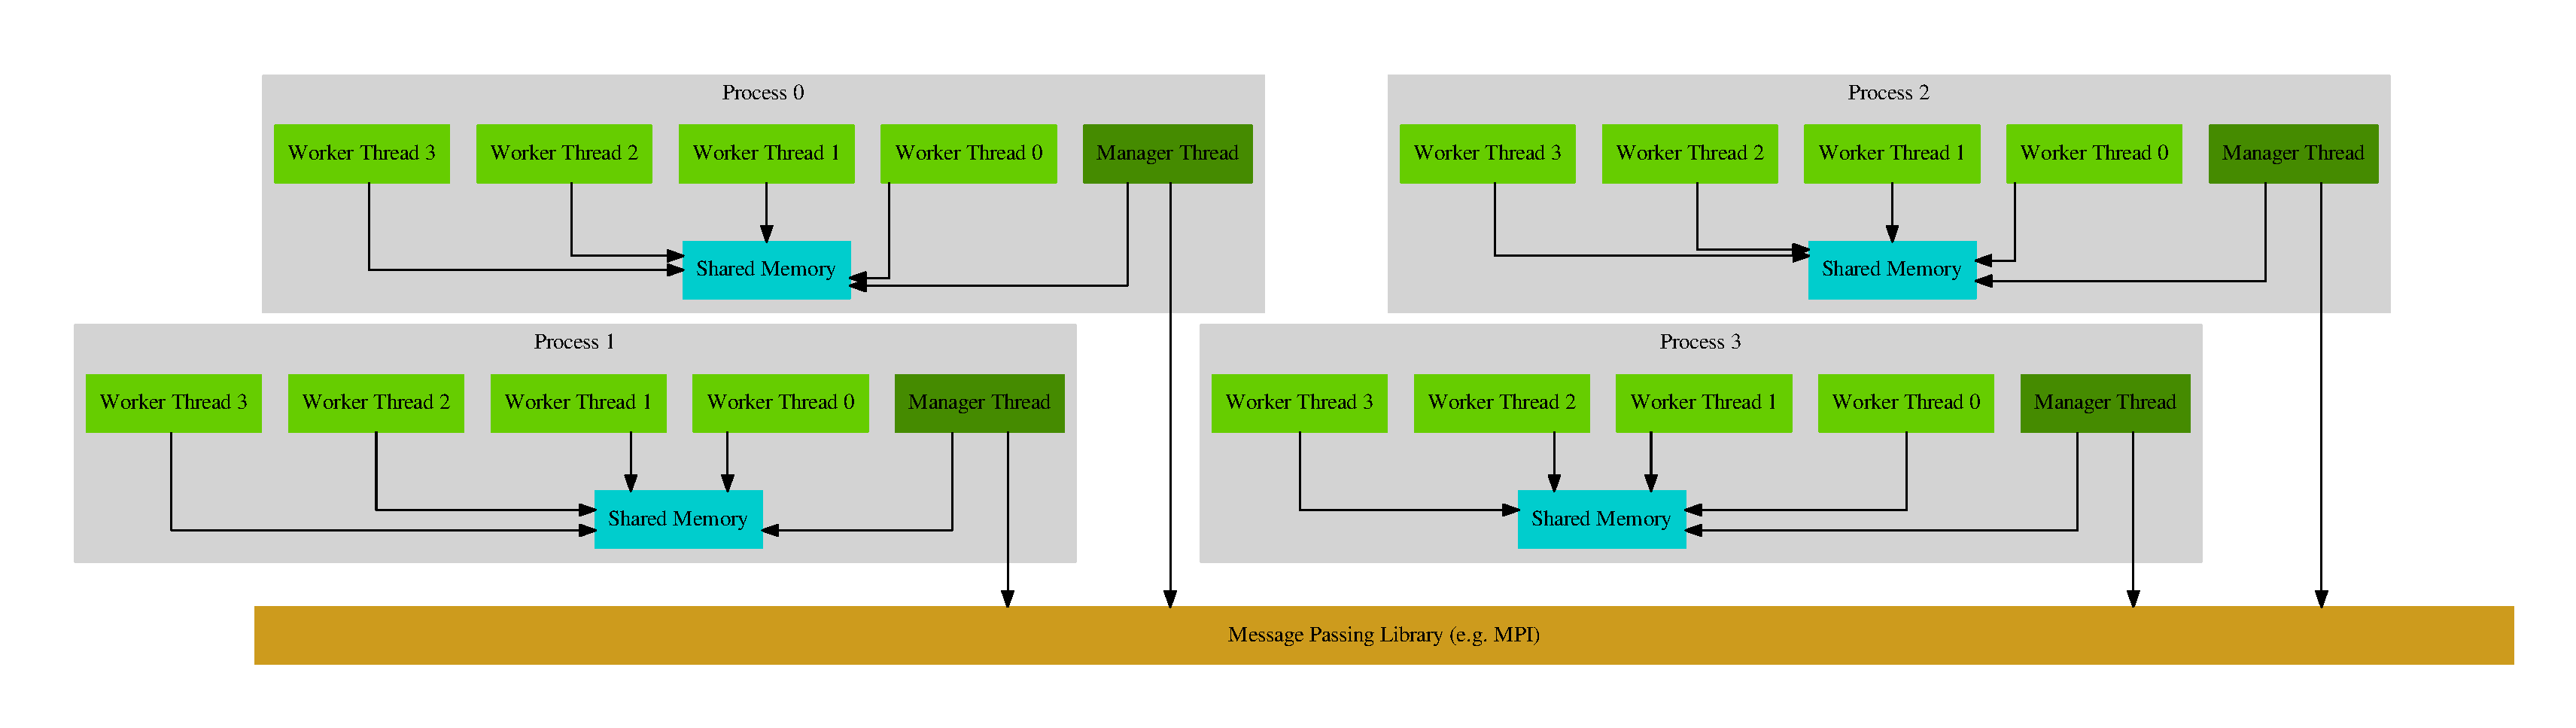
\includegraphics[width=1.2\textwidth]{../figs/graphviz/warped_communication.pdf}}
    Thread Message Passing Models
    \begin{itemize}
        \item Single threaded
        \item Funnelled
        \item Serialized
        \item Multiple
    \end{itemize}
\end{frame}

\begin{frame}{Communication Model: Traffic Model}
  \medskip
    \begin{block}{Intel\textsuperscript{\textregistered} Xeon\textsuperscript{\textregistered}
        E5410 (8 nodes)}
      \vspace*{-\medskipamount}
      \begin{footnotesize}
        \begin{itemize}
          \setlength{\itemsep}{-0.025in}
            \item Single: 1 thread (combining worker/manager threads)
            \item Others: 7 worker threads and manager thread
        \end{itemize}
      \end{footnotesize}
      \vspace{-\medskipamount}
        \begin{minipage}{0.55\textwidth}
            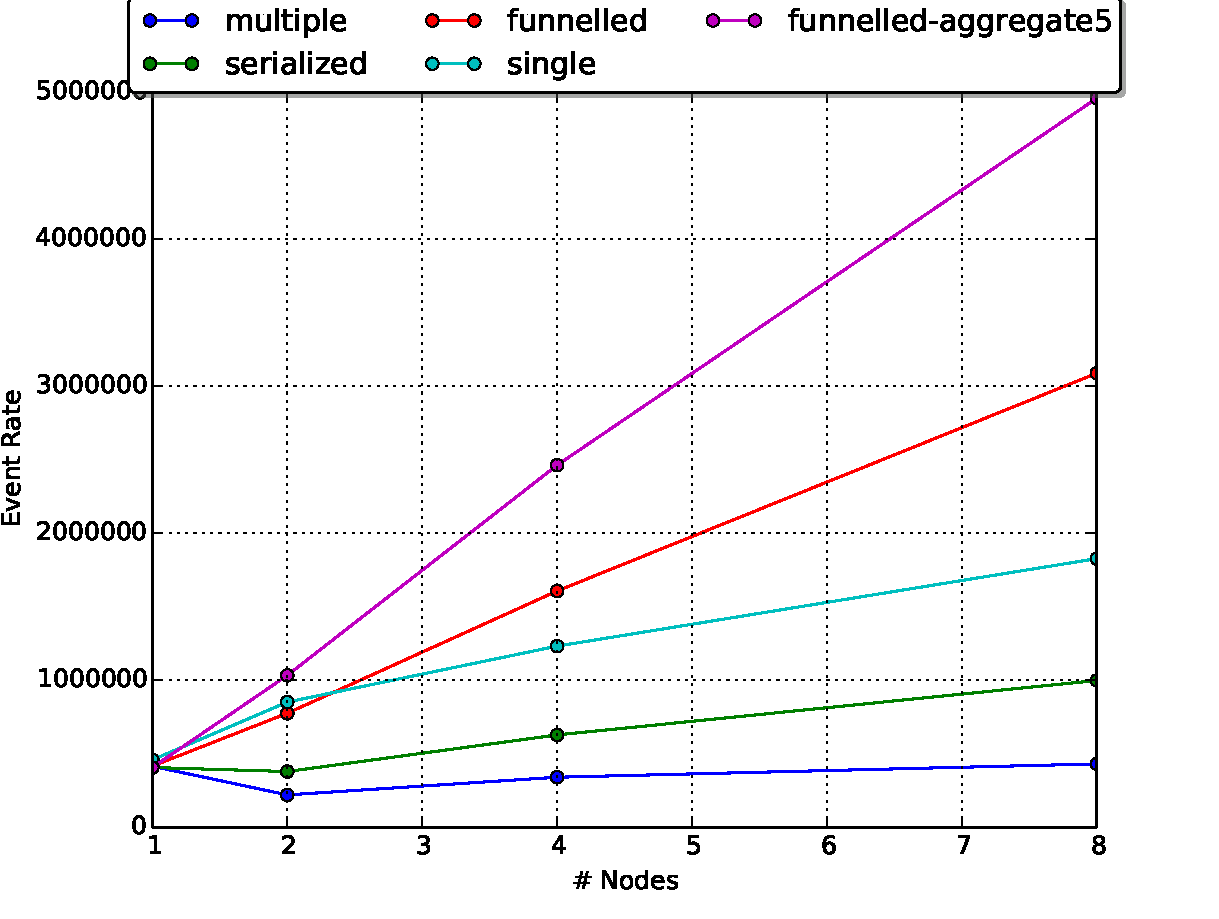
\includegraphics[width=\textwidth]{../figs/partitioning_communication/communication_traffic_eventrate.pdf}
        \end{minipage}%
        \begin{minipage}{0.55\textwidth}
            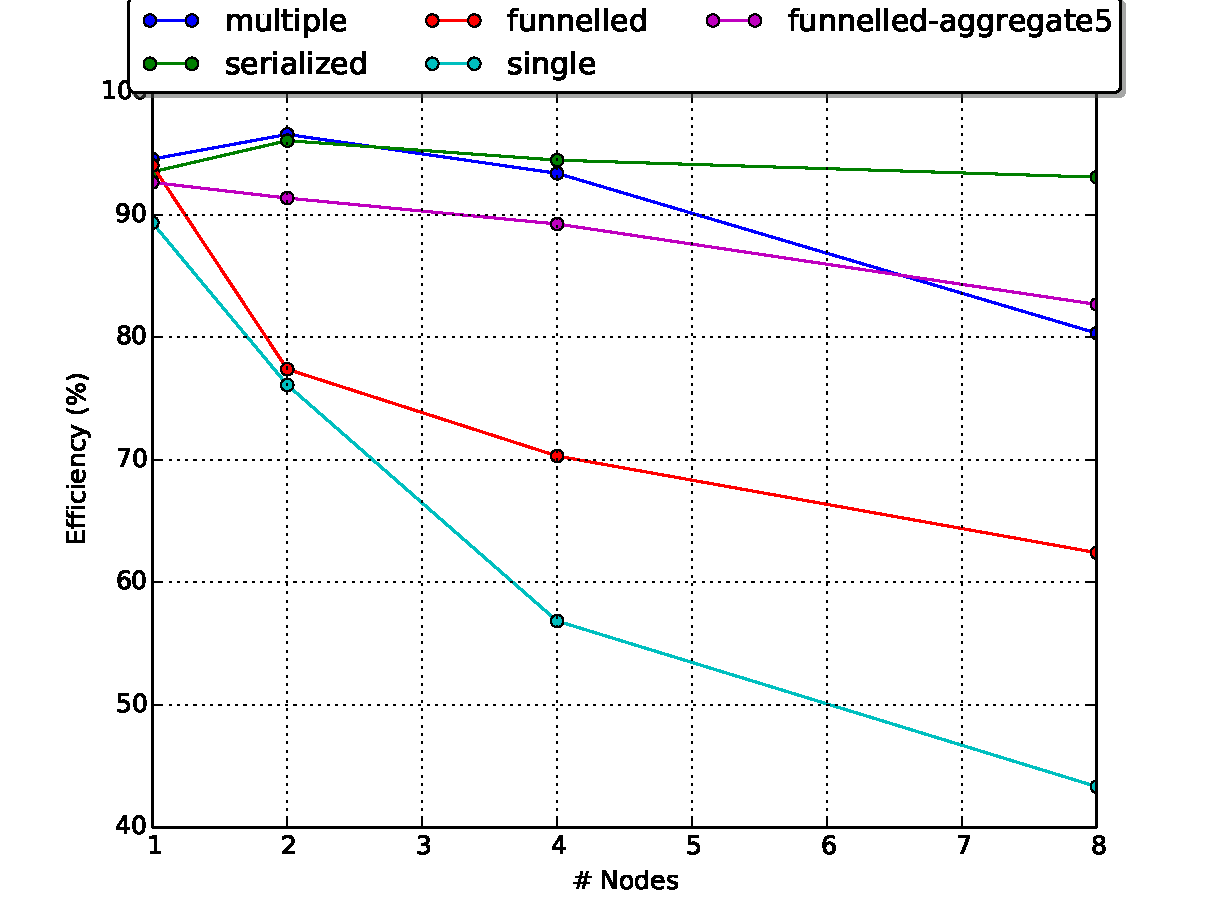
\includegraphics[width=\textwidth]{../figs/partitioning_communication/communication_traffic_efficiency.pdf}
        \end{minipage}
      \begin{footnotesize}
        \begin{itemize}
            \item Funneled/Single: Minimal Synchronization, High Latency
            \item Serialized/Multiple: Lots of Synchronization , Low Latency
            \item Performance will vary with model and partitioning.
        \end{itemize}
      \end{footnotesize}
    \end{block}
\end{frame}

\begin{frame}{Message Aggregation}
    \begin{itemize}
        \item Wait for $N$ messages with same \textbf{destination process} and send together

        \centerline{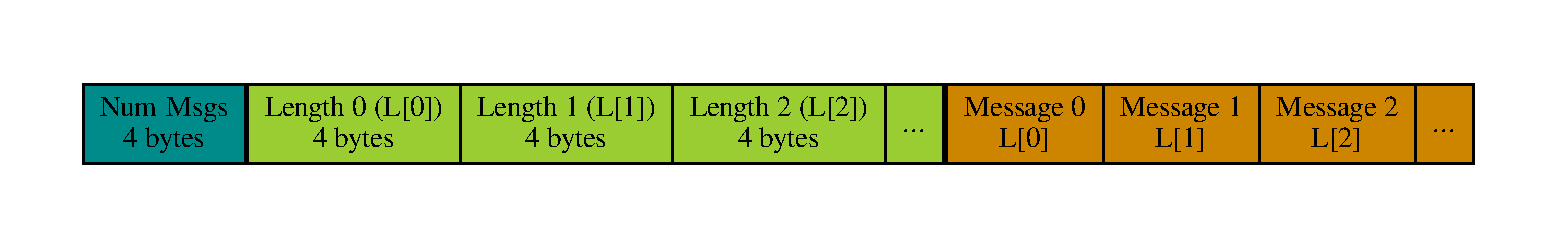
\includegraphics[width=1.25\textwidth]{../figs/graphviz/aggregation_format.pdf}}

        \item Pros
            \begin{itemize}
                \item Single buffer allocated for multiple messages
                \item Latency shared by multiple messages (TCP/IP/Ethernet/...)
                \item Events destined for same LP may be sent together
            \end{itemize}
            \bigskip
        \item Cons
            \begin{itemize}
                \item May increase event latency and increase receiver rollbacks
            \end{itemize}
    \end{itemize}
\end{frame}

\begin{frame}{Message Aggregation: Traffic Model}
    \begin{minipage}{0.5\textwidth}
        \centerline{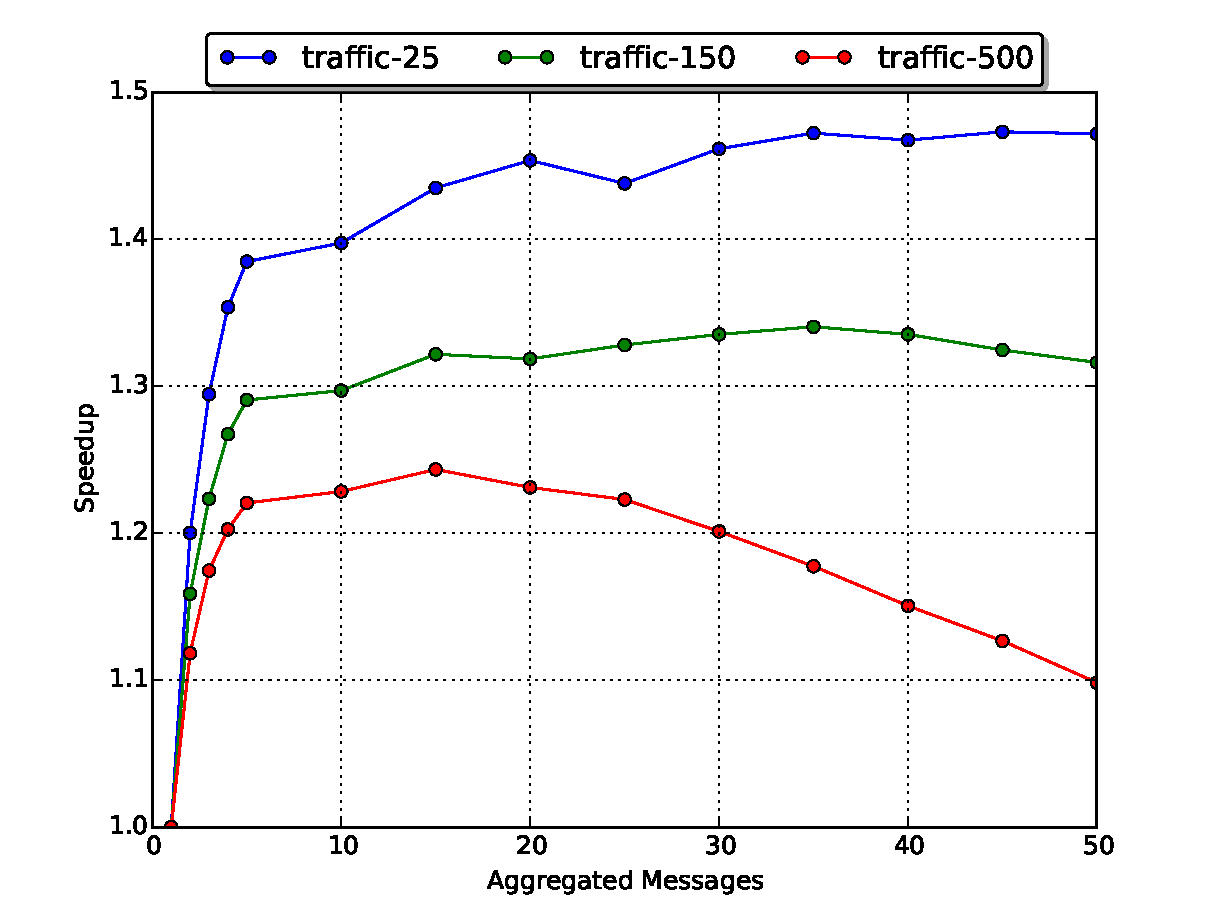
\includegraphics[width=1.1\textwidth]{../figs/partitioning_communication/aggregate_traffic_speedup.pdf}}
    \end{minipage}%
    \begin{minipage}{0.5\textwidth}
        \centerline{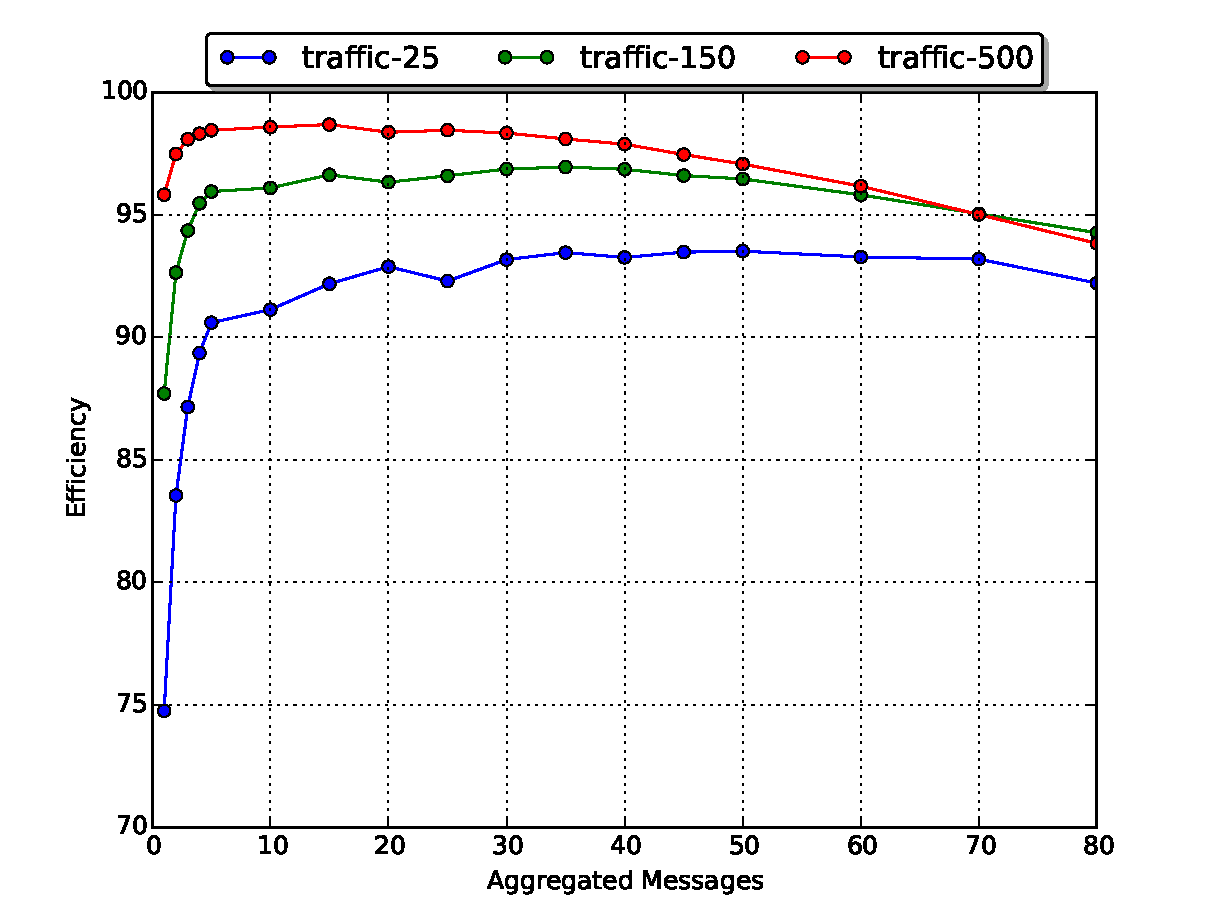
\includegraphics[width=1.1\textwidth]{../figs/partitioning_communication/aggregate_traffic_efficiency.pdf}}
    \end{minipage}
    \bigskip
    \begin{itemize}
        \item Best with small number of aggregated events
        \item Different behavior with different state saving periods
    \end{itemize}
\end{frame}

\begin{frame}{Message Aggregation: More Observations}

    \begin{columns}

    \begin{column}[t]{0.55\textwidth}
        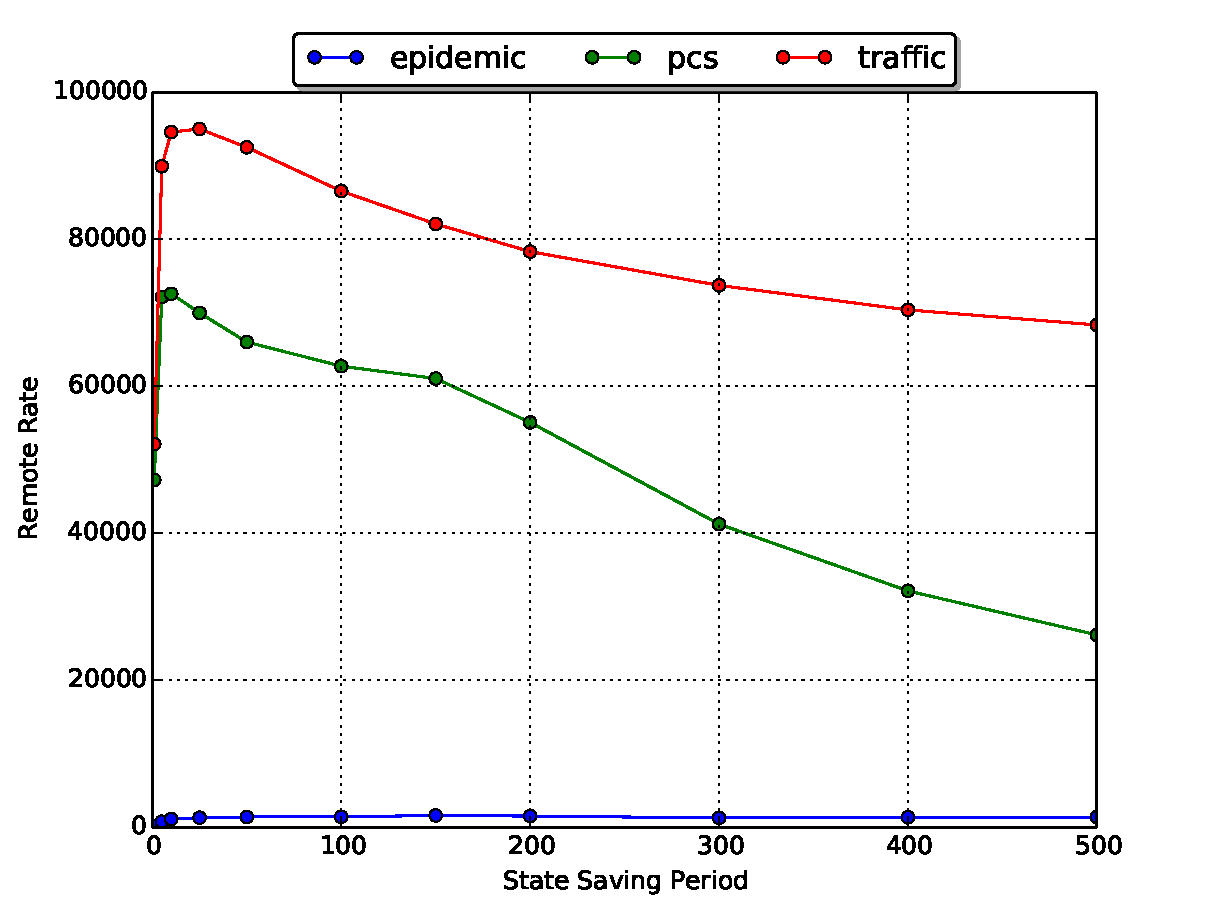
\includegraphics[width=\textwidth]{../figs/state_saving/beowulf/remote_rate.pdf}
        \vspace*{-\bigskipamount}
        \begin{small}
        \begin{itemize}
            \item Faster rate of remote events better
        \end{itemize}
        \end{small}
    \end{column}

    \begin{column}[t]{0.55\textwidth}
        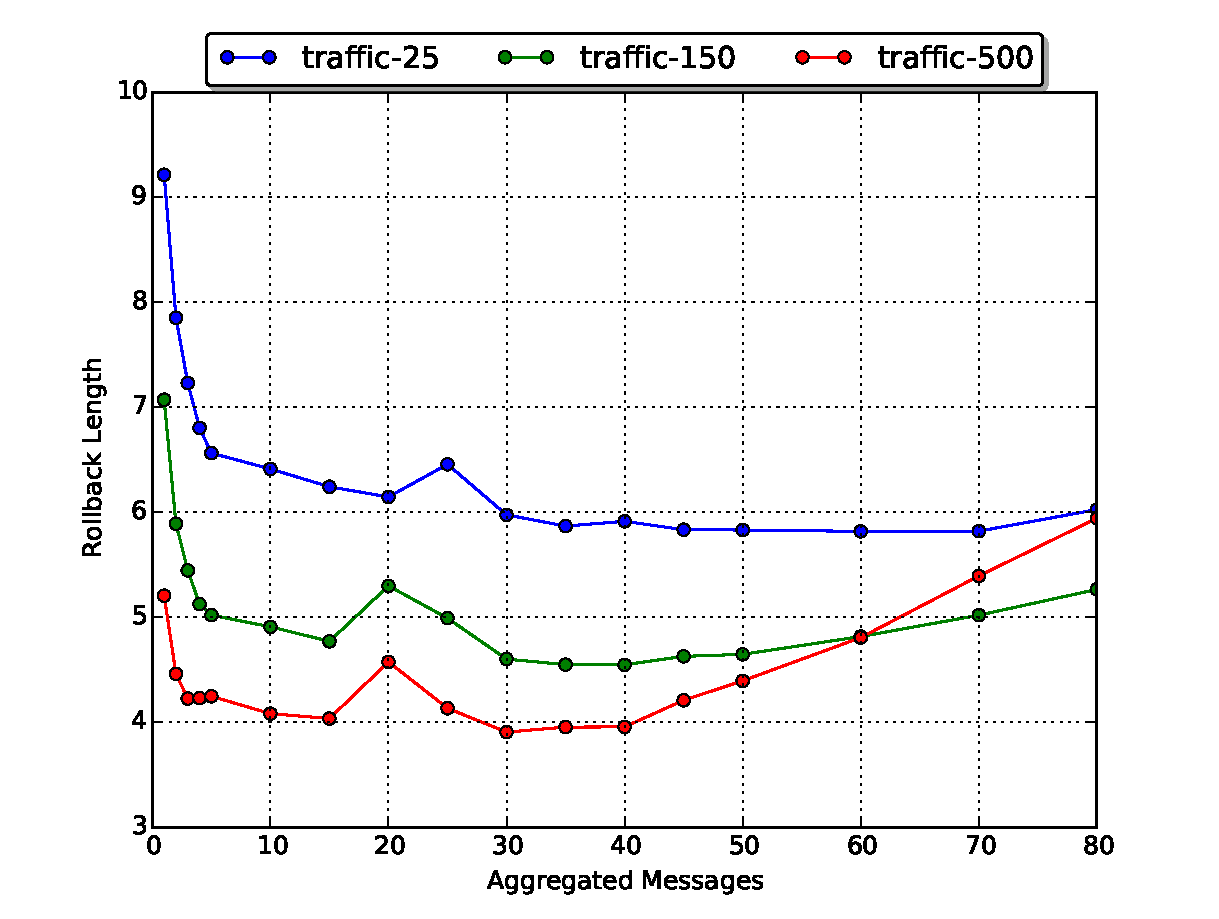
\includegraphics[width=\textwidth]{../figs/partitioning_communication/aggregate_traffic_rblength.pdf}
        \vspace*{-\bigskipamount}
        \begin{small}
        \begin{itemize}
            \item Can lower rollback length?
        \end{itemize}
        \end{small}
    \end{column}

    \end{columns}

    \bigskip
    \bigskip

    $AverageRollbackLength = RolledBackEvents/Rollbacks$

\end{frame}

\begin{frame}{Memory Allocation: Traffic Model}
  \medskip
    \begin{block}{Intel\textsuperscript{\textregistered} Xeon\textsuperscript{\textregistered} X5675
        (6 cores/up to 12 threads)}
        \begin{columns}
        \begin{column}{0.7\textwidth}
            \smallskip
            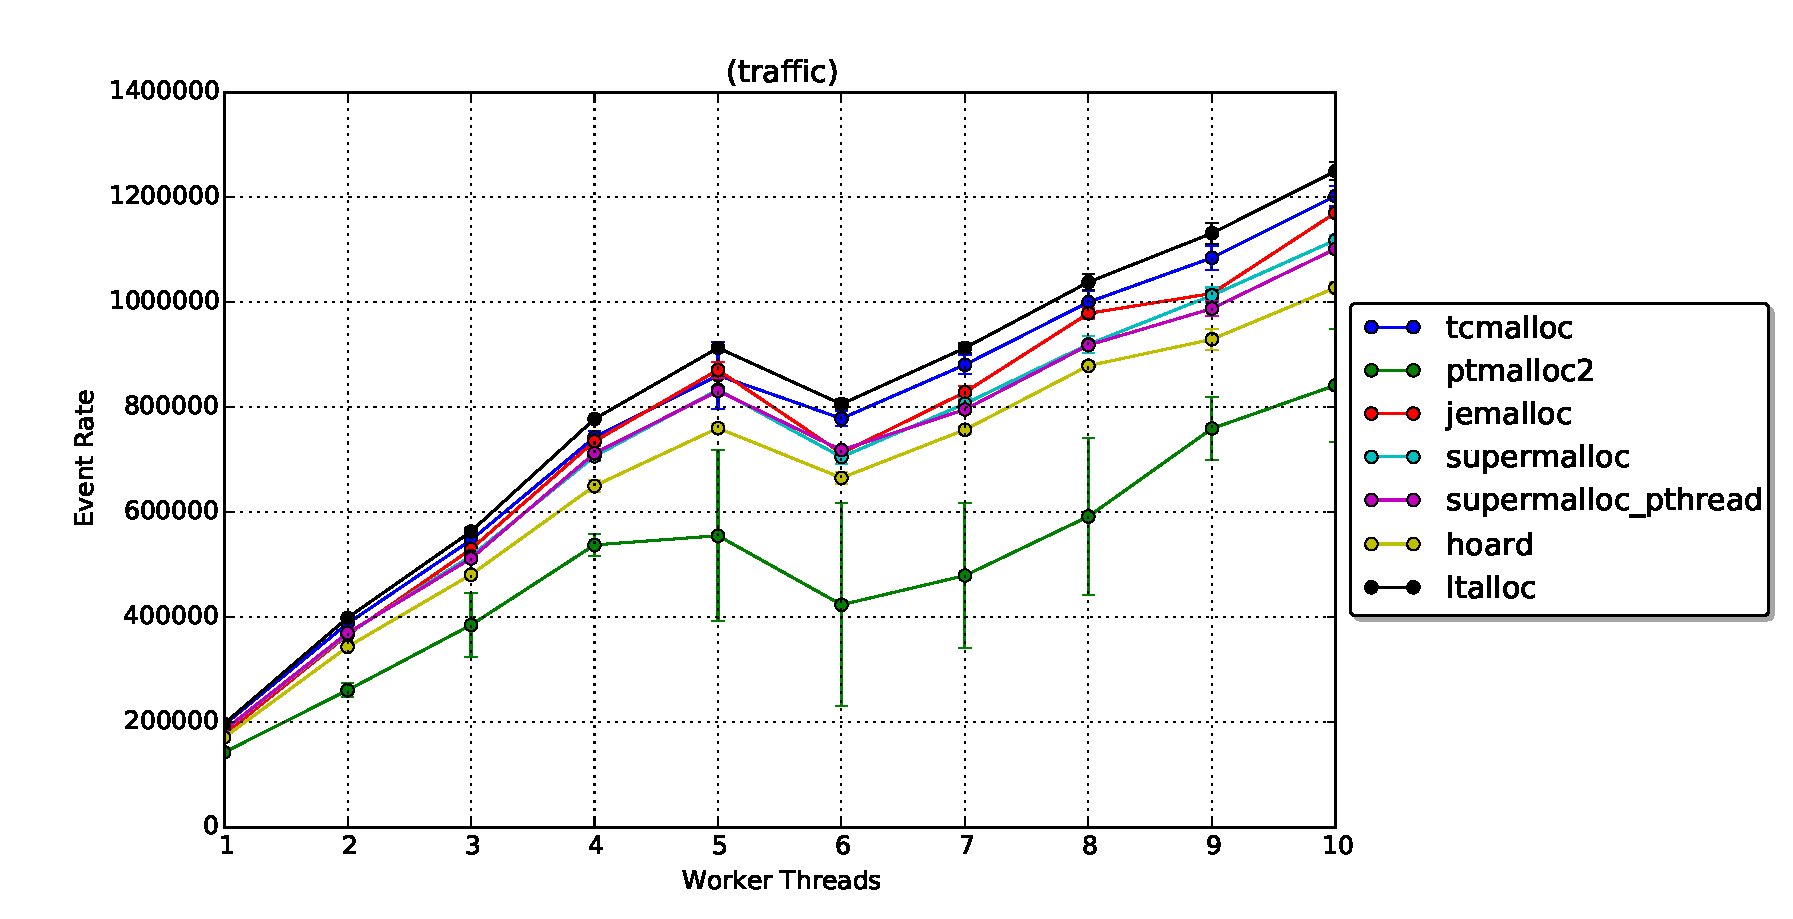
\includegraphics[width=\textwidth]{../figs/memory_allocation/traffic_eventrate.pdf} \\[-0.15in]
            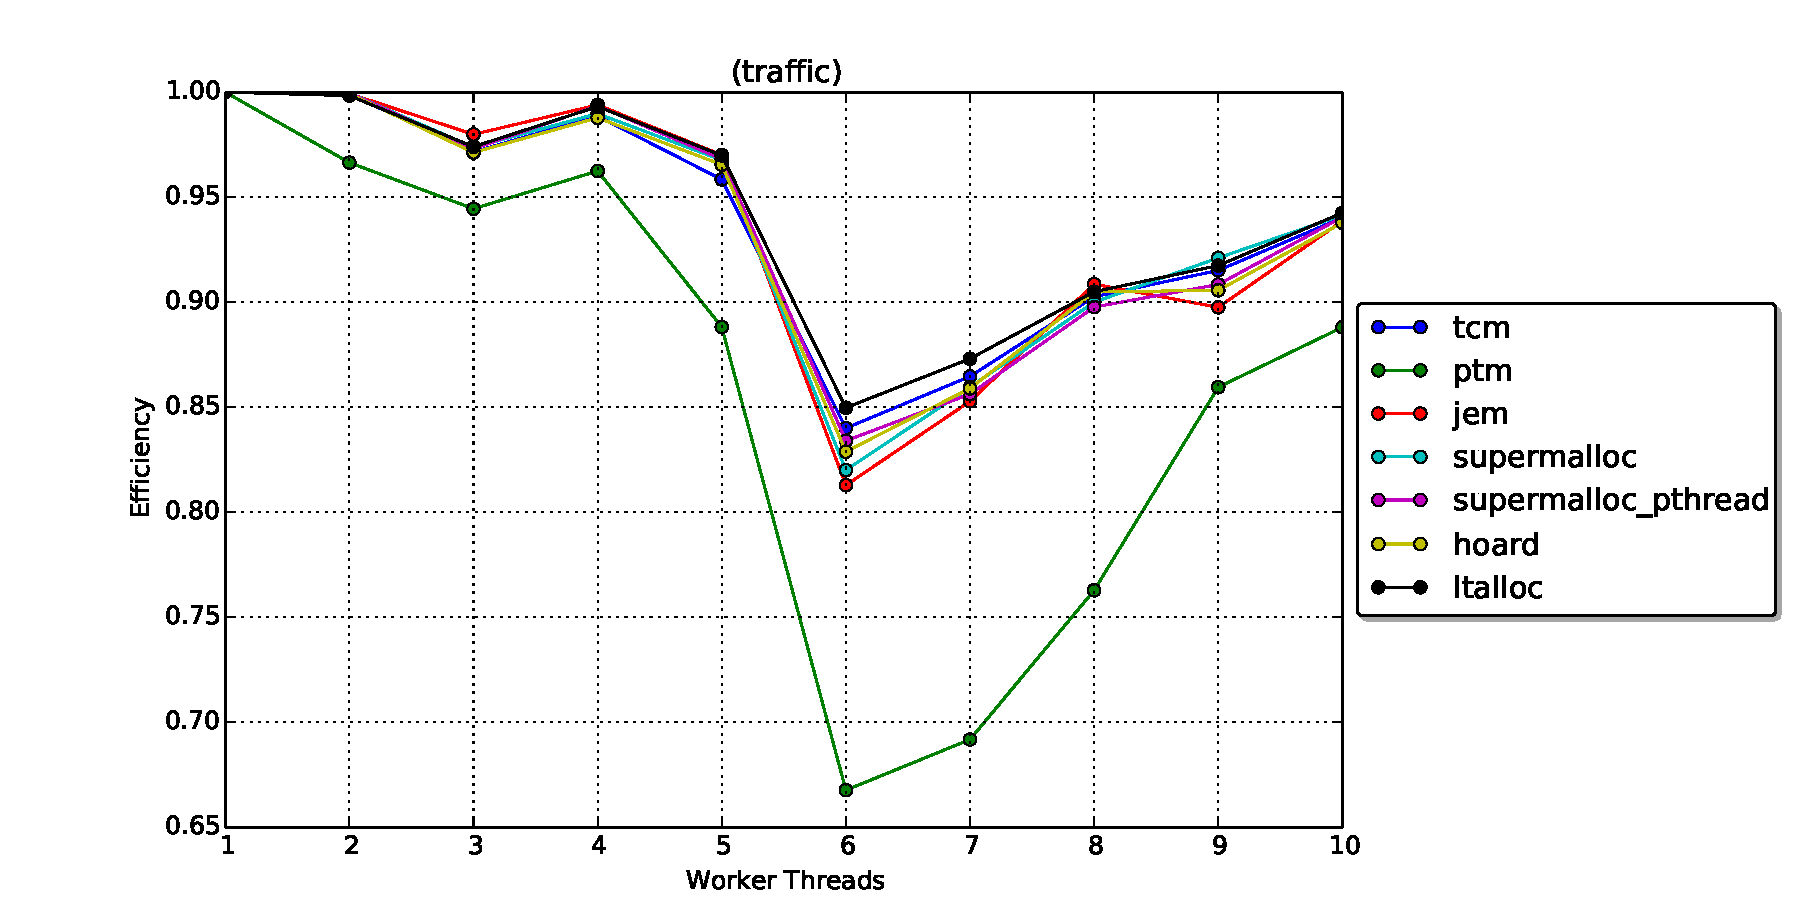
\includegraphics[width=\textwidth]{../figs/memory_allocation/traffic_efficiency.pdf}
        \end{column}
        \begin{column}{0.3\textwidth}
          \begin{small}
            \begin{itemize}
                \item Imbalance at 6 worker threads
                  \bigskip
                  \bigskip
                \item ptmalloc2 (the default in GLIBC) is inefficient and unpredictable
            \end{itemize}
          \end{small}
        \end{column}
        \end{columns}
    \end{block}
\end{frame}

\begin{frame}{Scaling Simulation Models: Advantages}
    \begin{block}{Intel\textsuperscript{\textregistered} Xeon\textsuperscript{\textregistered}
        E5410 (8 nodes/7 worker threads)}\end{block}
    \begin{minipage}{0.5\textwidth}
        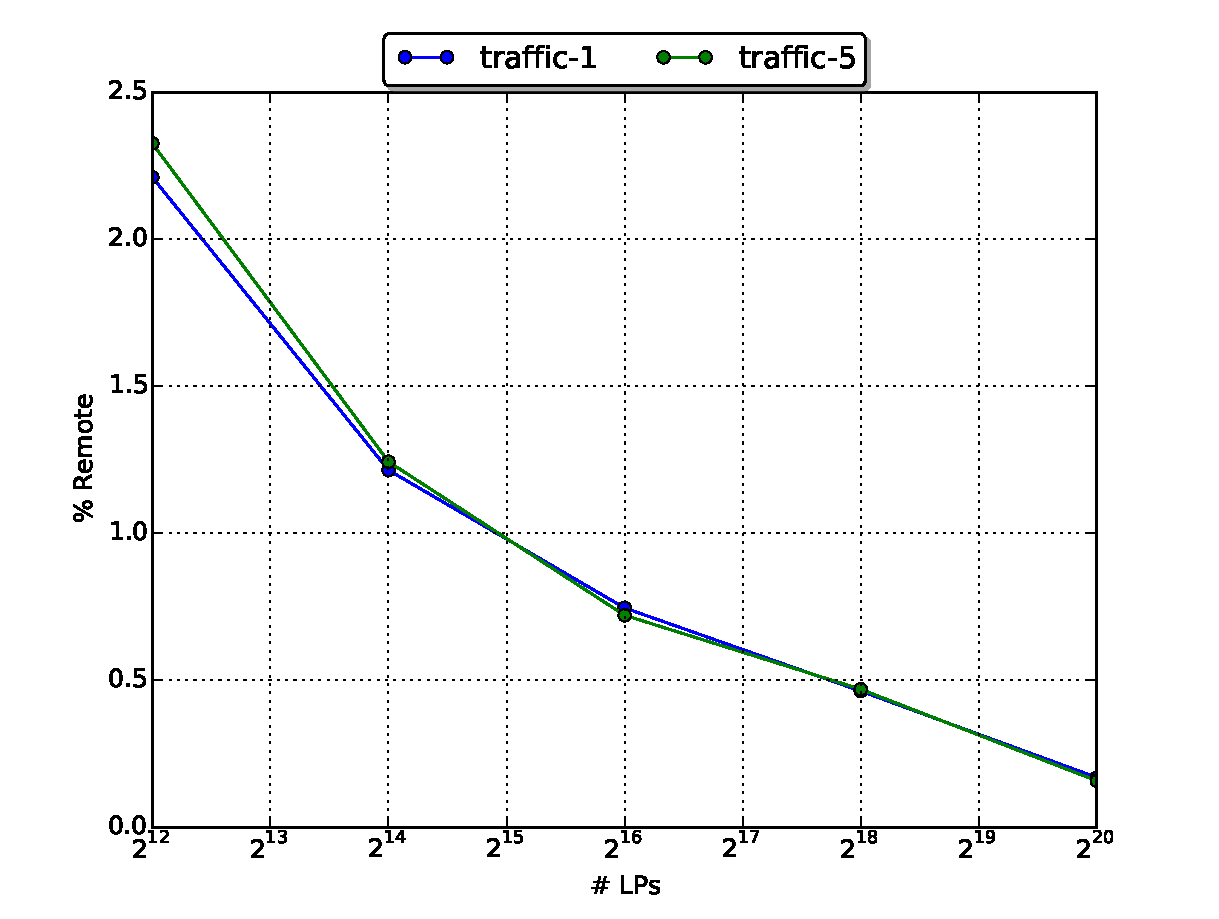
\includegraphics[width=1.1\textwidth]{../figs/scale/scale_premote_traffic.pdf}
    \end{minipage}%
    \begin{minipage}{0.5\textwidth}
        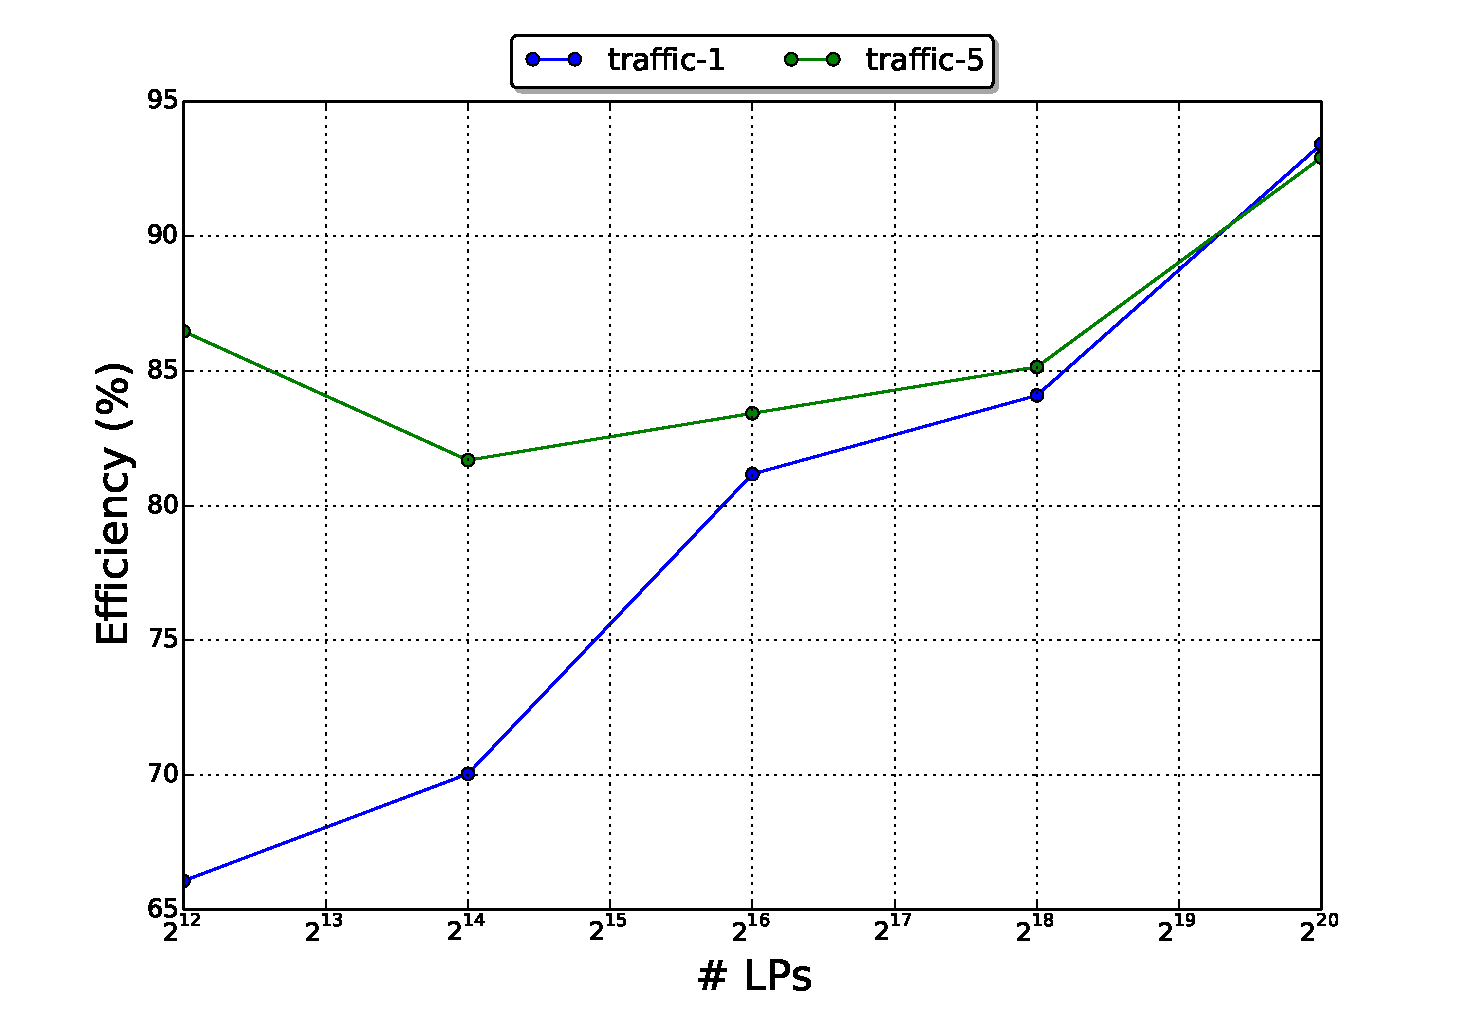
\includegraphics[width=1.1\textwidth]{../figs/scale/scale_efficiency_traffic.pdf}
    \end{minipage}
    \begin{itemize}
        \item Coarser Granularity
        \item Higher Efficiency
    \end{itemize}
\end{frame}

\begin{frame}{Scaling Simulation Models: Disadvantages}
    \begin{block}{Intel\textsuperscript{\textregistered} Xeon\textsuperscript{\textregistered}
        E5410 (8 nodes/7 worker threads)}\end{block}
    \begin{minipage}{0.5\textwidth}
        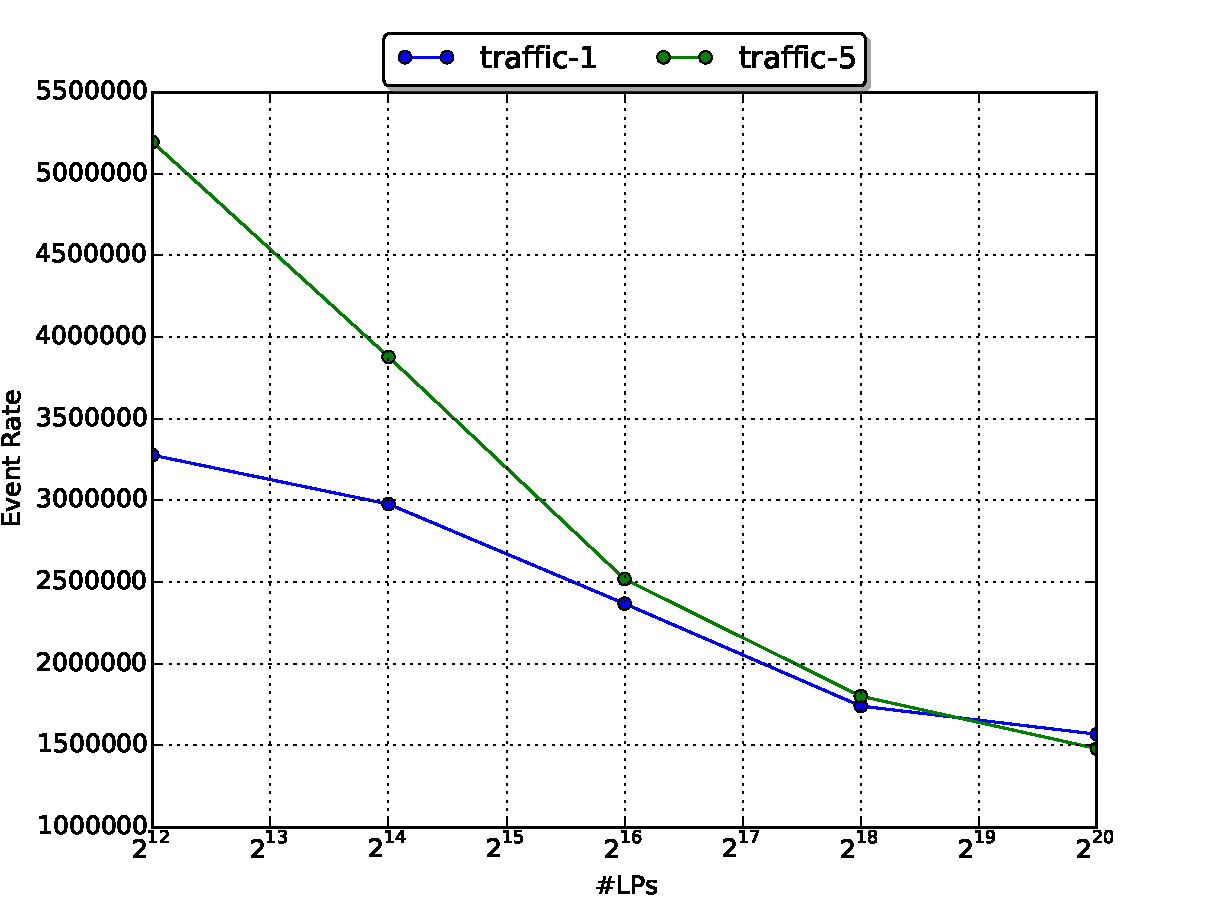
\includegraphics[width=\textwidth]{../figs/scale/scale_event_rate_traffic.pdf}
    \end{minipage}%
    \begin{minipage}{0.5\textwidth}
        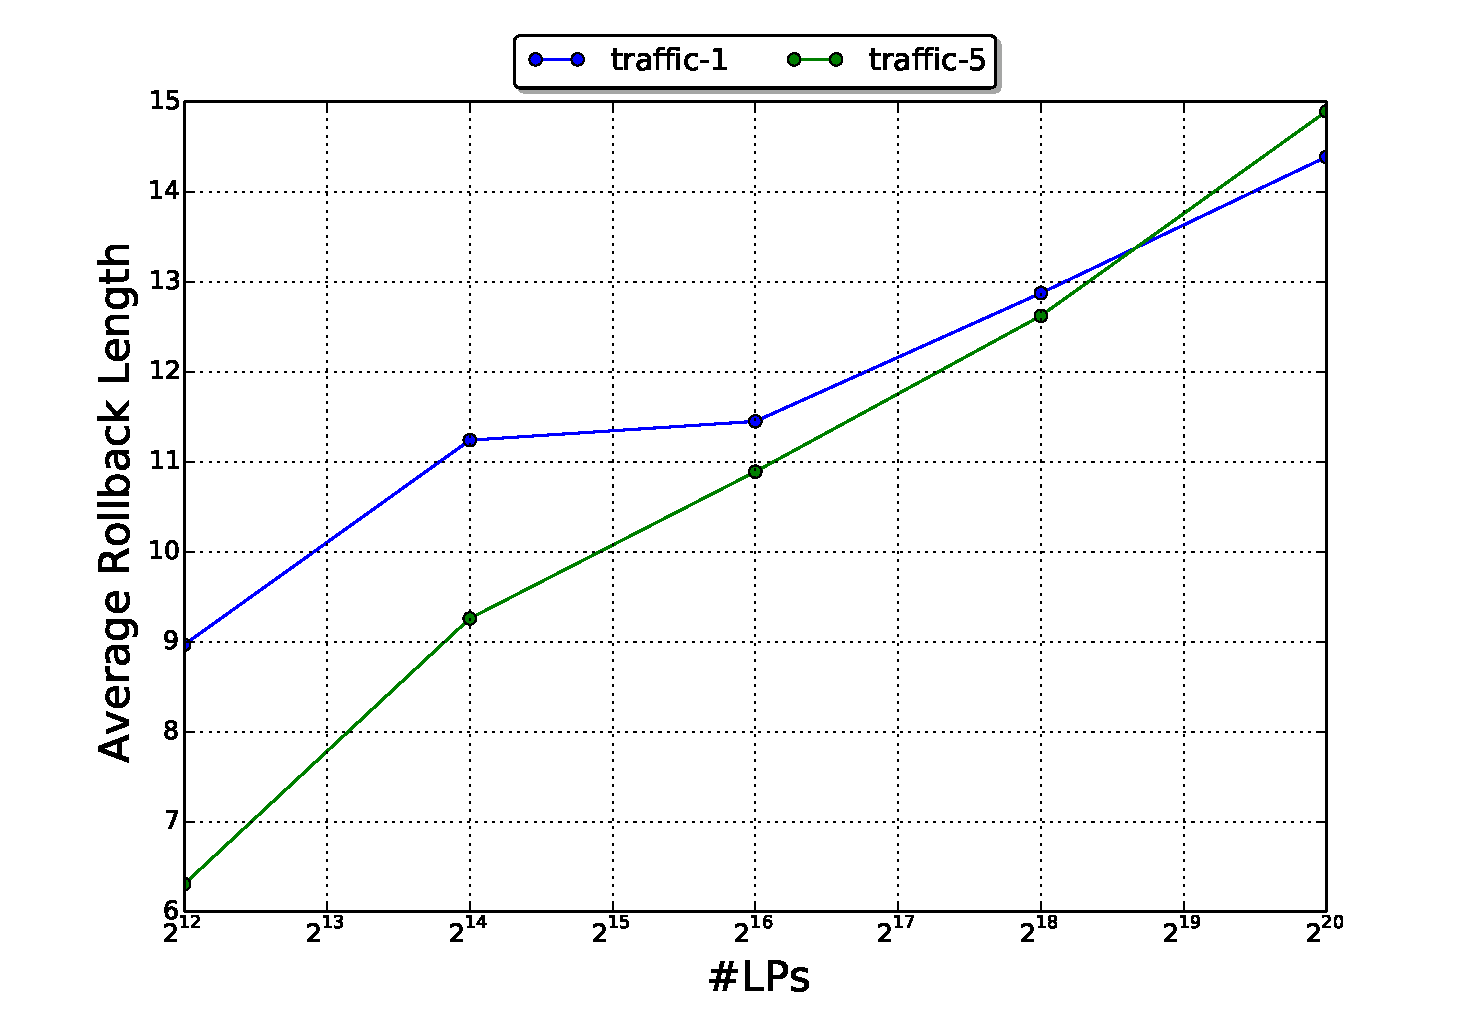
\includegraphics[width=\textwidth]{../figs/scale/scale_arl_traffic.pdf}
    \end{minipage}
    \begin{itemize}
        \item More LPs to fossil collect
        \item Longer Rollbacks
    \end{itemize}
\end{frame}

\begin{frame}{Conclusions \& Future Research}
    \begin{itemize}
        \item Conclusions
            \begin{itemize}
                \item Synchronization should always be avoided
                    \begin{itemize}
                        \item Interprocess communication: Higher latency over synchronization
                        \item 1 LTSF queue per worker thread
                    \end{itemize}
                \smallskip

                \item Avoid communication ... If possible
                    \begin{itemize}
                        \item If it cannot be avoided, aggregating messages may help
                        \item Hard to calculate GVT efficiently
                        \item Memory consumption: May need flow control
                    \end{itemize}
                \smallskip

                \item Alternative multi-threaded memory allocators better than GLIBC default
            \end{itemize}
        \bigskip

        \item Future Research
            \begin{itemize}
                \item Optimistic Fossil Collection
                \item Scaling up
            \end{itemize}
    \end{itemize}
\end{frame}

\end{document}

